\chapter{相关工作}

为了更好地设计适用于日常健康场景下的面诊系统,本章将介绍当前比较流行的基于面诊技术的面诊系统设计,最后简单介绍本文的研究方法。

\section{面诊系统}

面诊系统是基于面诊算法为用户提供面诊功能的一套系统。
目前已经有不少研究将面诊技术落地,下面将主要介绍代表性的几类,同时简单概括其特点以及不足之处。

\begin{figure}[h]
    \centering
    \subfigure[面诊仪]{
        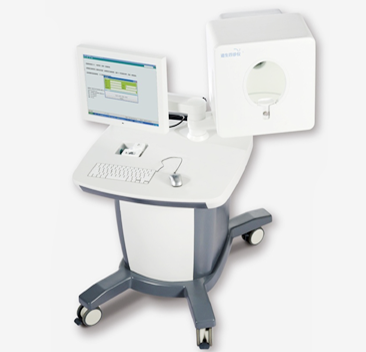
\includegraphics[height=6cm]{images/mzy.png}
    }
    \subfigure[云中医智能镜]{
        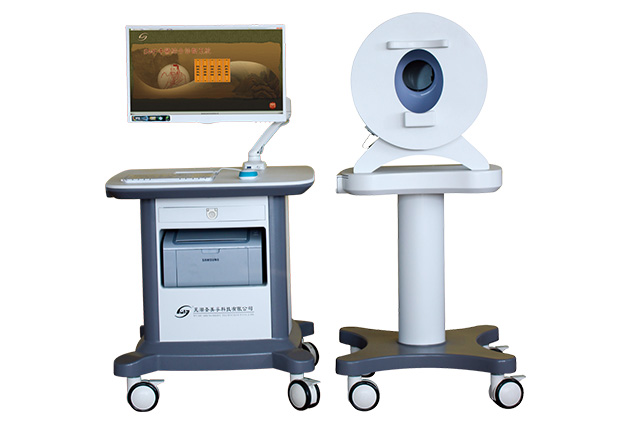
\includegraphics[height=6cm]{images/SMF.jpg}
    }
    \caption{面诊仪}
    \label{fig:med}
\end{figure}

\subsection{面诊仪}
目前面诊技术最主要的应用场景是医疗环境中的各类面诊仪。面诊仪如舌面象仪可作为初步信息采集工具得到患者的面色,舌象等信息,而面色自动识别分析系统则能得出初步的诊断结果,然后由医生根据这些信息得到最终结果\cite{崔骥2018人工智能背景下中医诊疗技术的应用与展望}。
面诊仪如道生面诊仪\cite{邸丹2016手持式舌象仪的研制}是目前某些医院用来采集面部信息的设备, 芜湖圣美孚科技有限公司\footnote{http://www.smfkj.com/}也有一款舌面诊一体化设备,
这类系统可以实现面部图像采集以及面部特征提取,如面色、唇色、舌苔、舌象等,为诊断提供依据。

但面诊仪主要是医疗环境中使用,不适合日常场景下:这类面诊系统因为依赖特有的设备,操作比较复杂,需要在中医医师的指导下,进行舌相面色诊断信息采集,最终结果需要中医医师进行判断。
此外,当前技术发展非常迅速,当新的面诊算法出现时,面诊仪没有合适的算法更新和添加机制,设备迭代成本较大。

\subsection{云中医}

\begin{figure}
    \centering
    \subfigure[云中医智能镜]{
        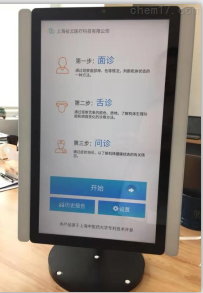
\includegraphics[width=4.5cm]{images/yzy.png}
    }
    \subfigure[云中医诊断机器人]{
        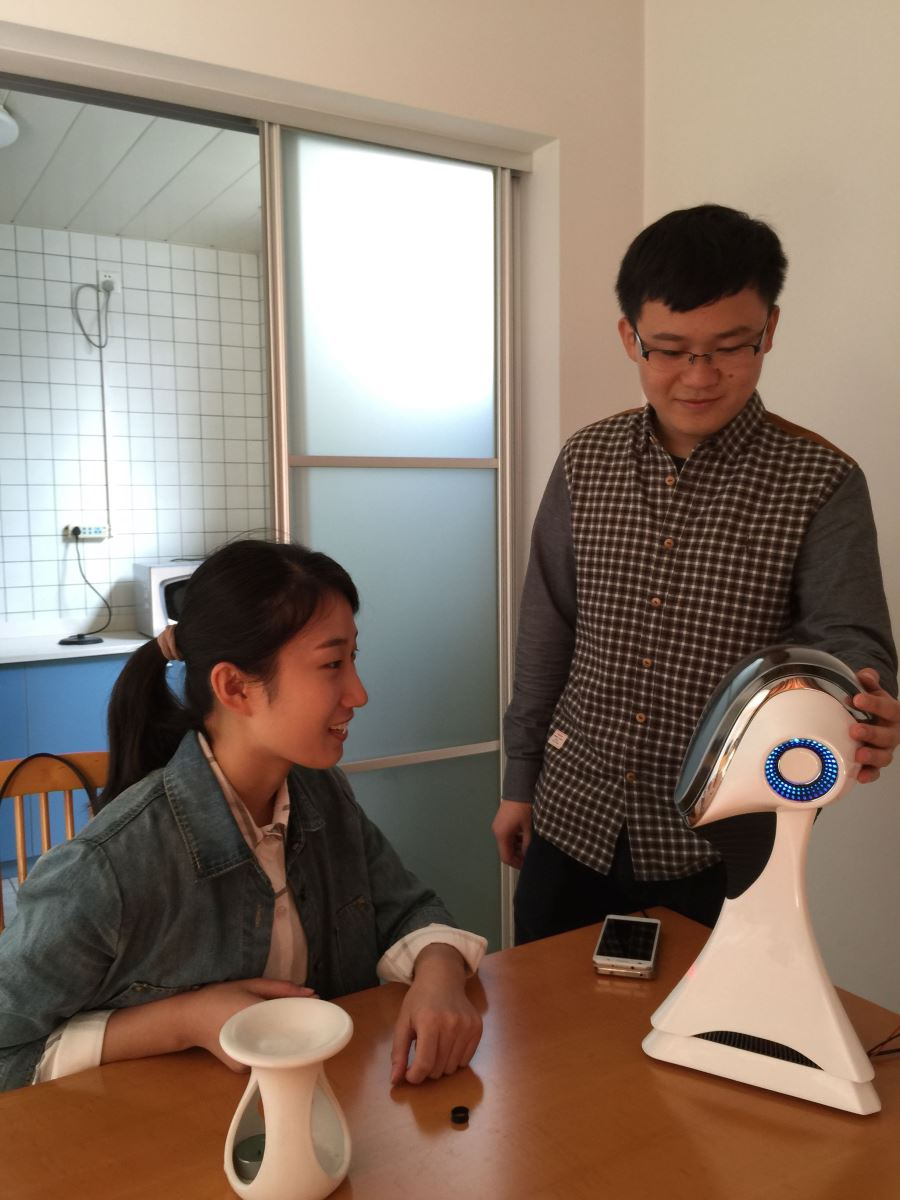
\includegraphics[width=4.5cm]{images/med_robot.jpg}
    }
    \subfigure[云中医应用]{
        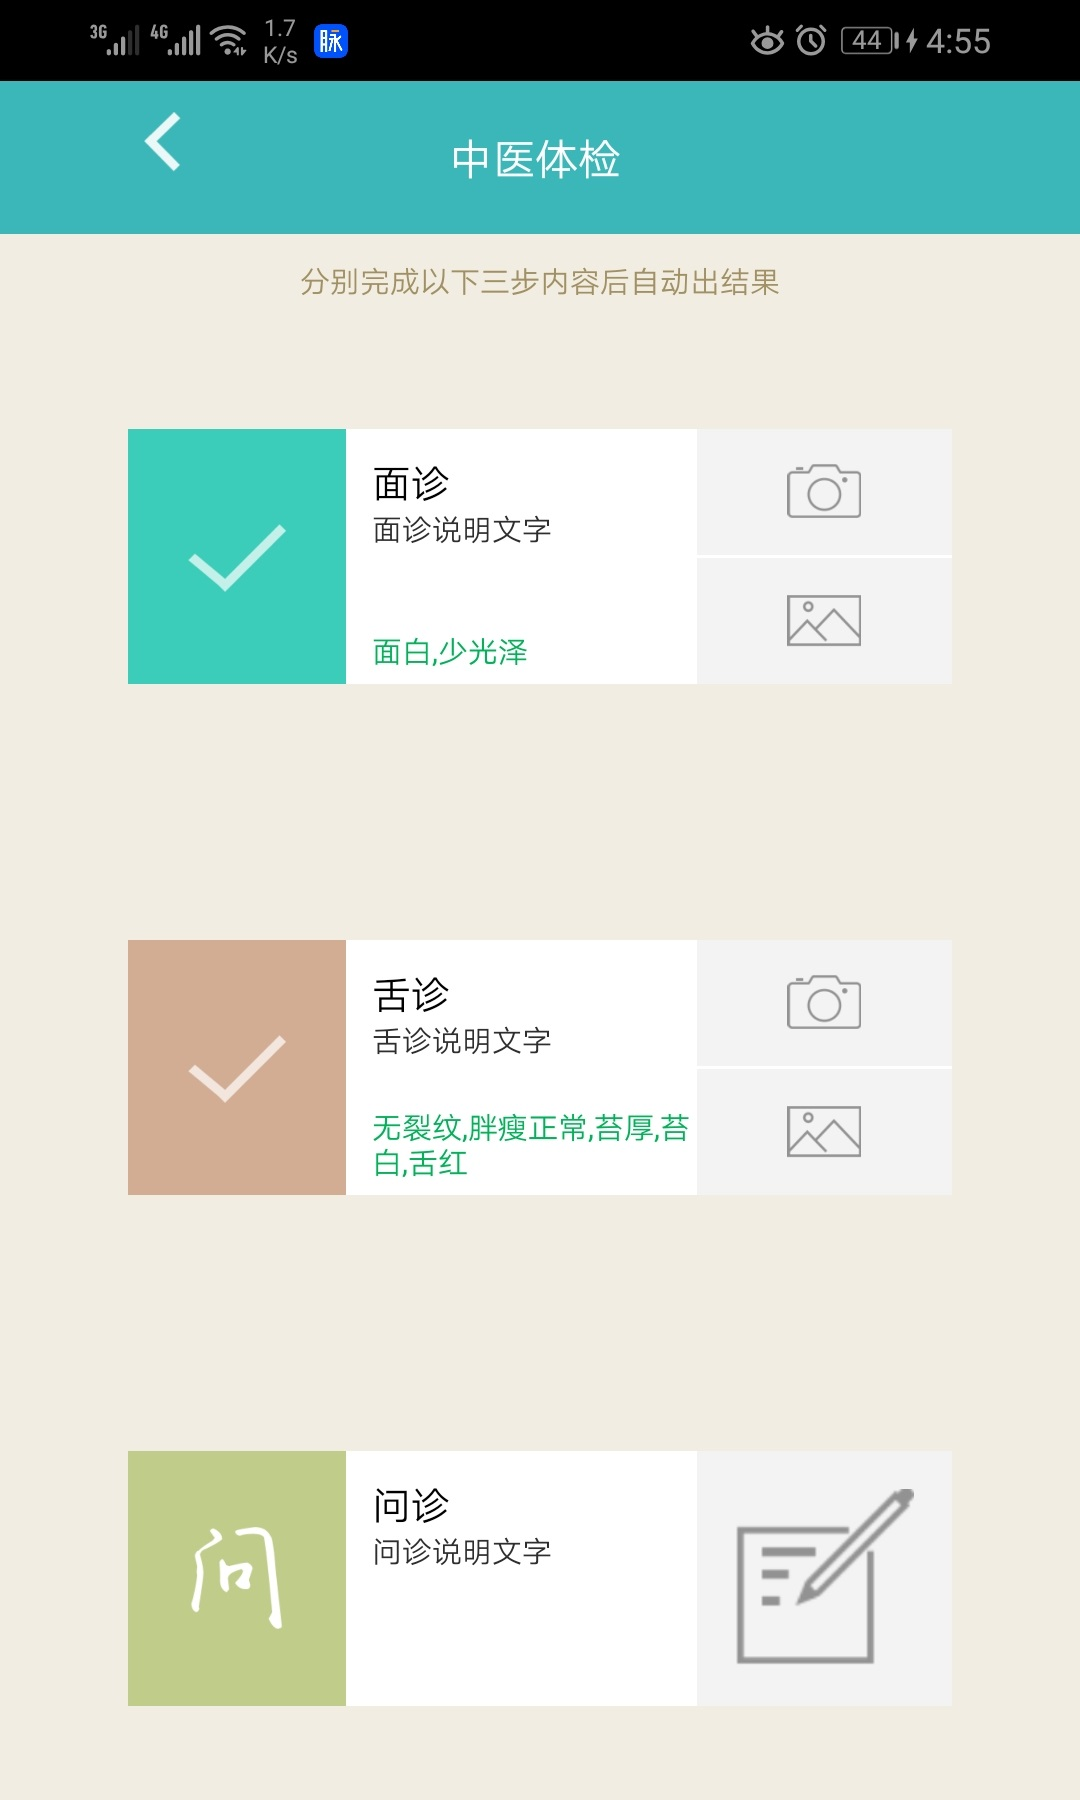
\includegraphics[width=4.5cm]{images/main1.jpg}
    }
    \caption{云中医系列产品}
    \label{fig:cloudmed}
\end{figure}

云中医是复旦大学计算机学院张文强老师和上海中医药大学合作开发的一款面诊应用,旨在为用户提供一个方便的自我诊断和健康管理平台,目前主要应用场景是各大社区、诊所给用户做健康参考。该应用以中医面诊、舌诊、问诊理论为指导,在手机上模拟实现了诊断的过程:用户需要依次对自己的面部和舌头进行拍照,回答一些与自己健康状况相关的问题,最终会收到一份完整的健康报告和一些健康建议。

\begin{figure}[h]
    \centering
    \subfigure[主界面]{
        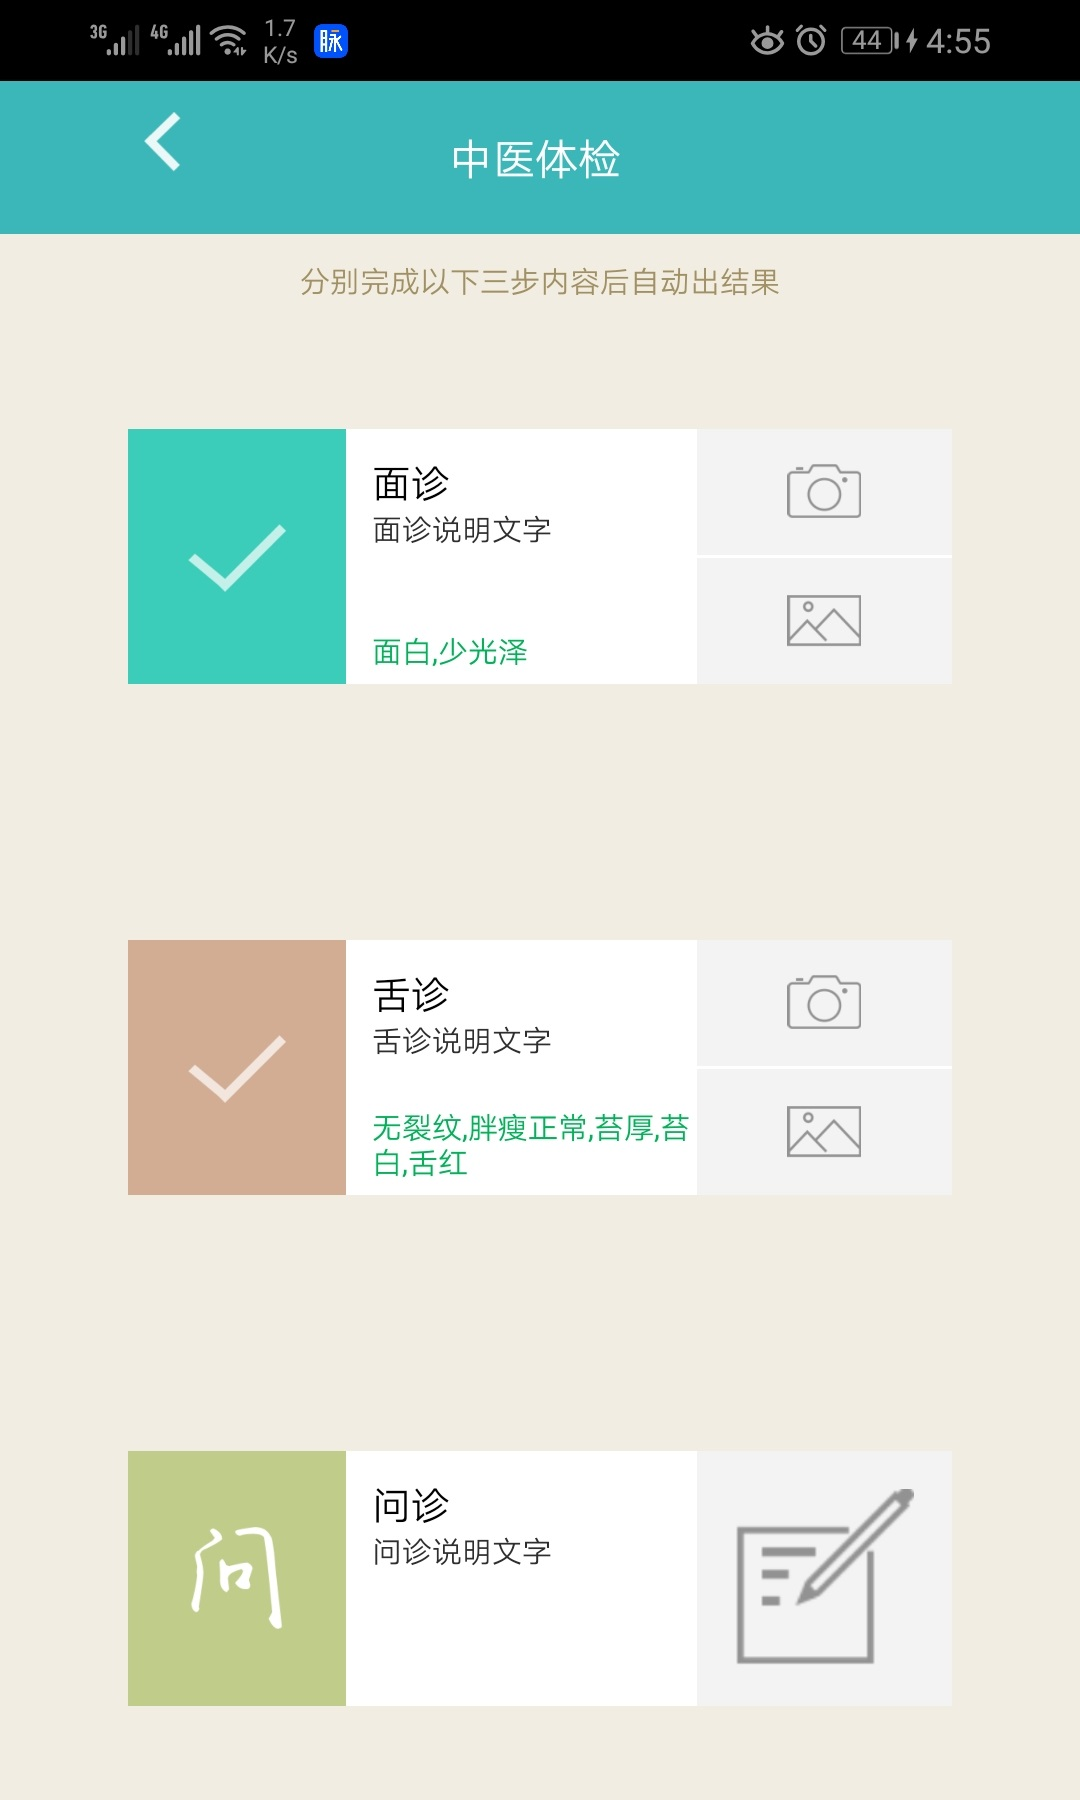
\includegraphics[width=4.5cm]{images/main1.jpg}
    }
    \subfigure[问诊]{
        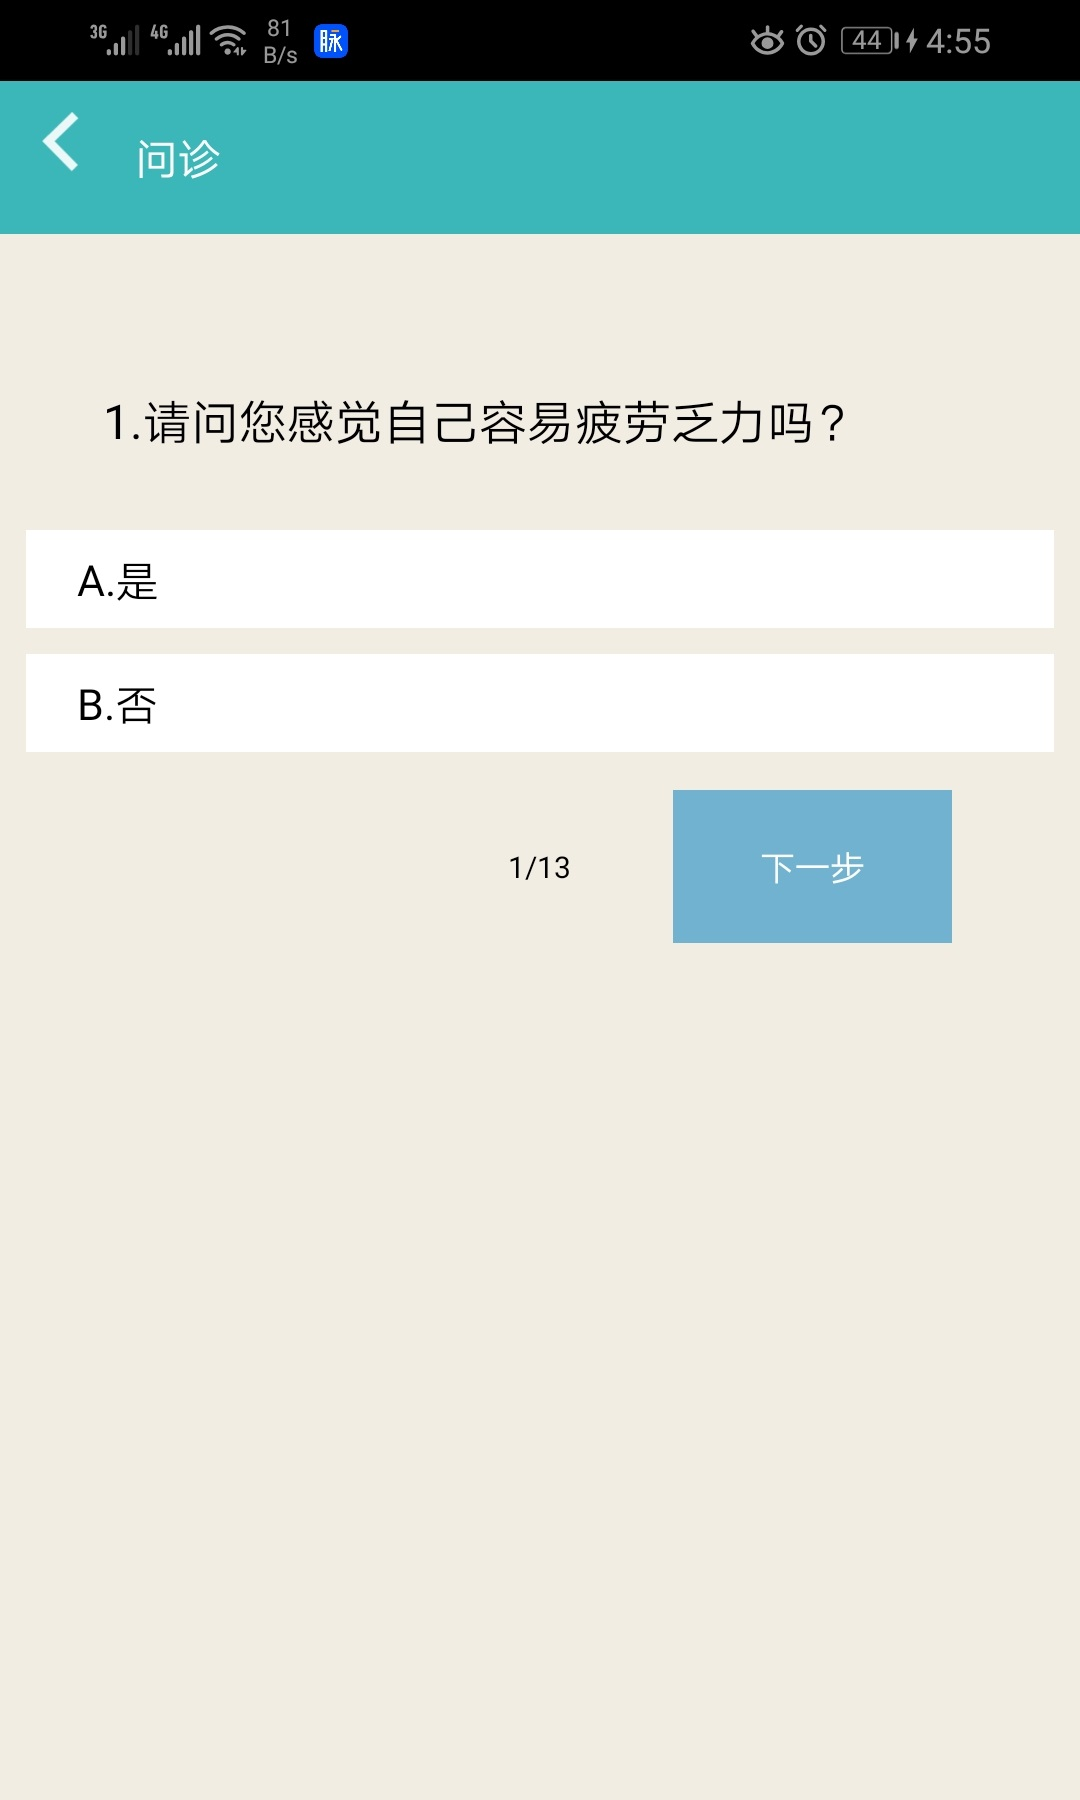
\includegraphics[width=4.5cm]{images/main2.jpg}
    }
    \subfigure[健康报告]{
        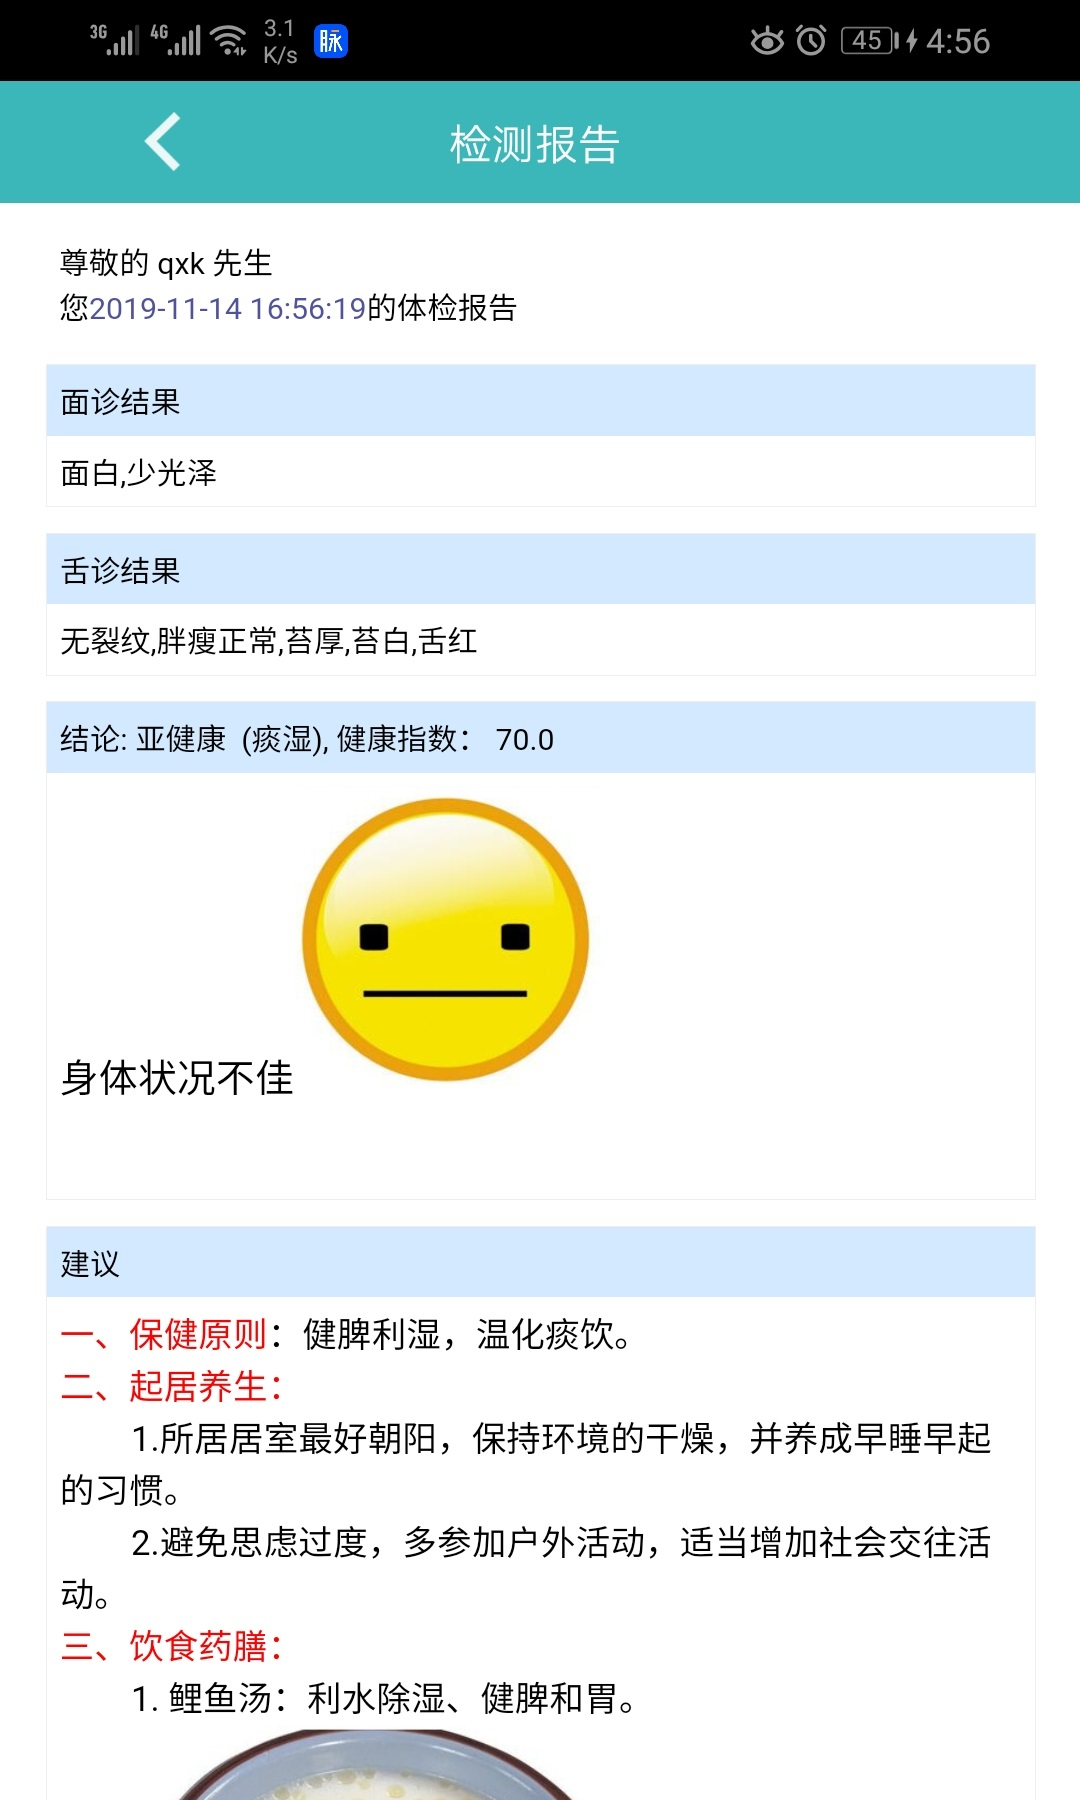
\includegraphics[width=4.5cm]{images/main3.jpg}
    }
    \caption{云中医主要界面}
    \label{fig:main}
\end{figure}

云中医应用的主要界面及使用流程如图 \ref{fig:main}所示:用户进入诊断页面之后,会看到三个区域:面诊、舌诊、问诊。面诊和舌诊通过拍照或者上传图片完成,问诊是通过依次回答13个问题来完成。依次完成面诊、舌诊、问诊后,系统会给出用户的体质和健康分数,并且给出对应的健康建议。
s
云中医\cite{张红凯2018基于舌}的系统设计对设备要求比较灵活,在移动设备、机器人平台上都有对应的产品,其中包括云中医诊断机器人\footnote{http://www.sohu.com/a/135358060\_205169/},云中医智能镜,云中医应用等,但是遗憾的是,云中医虽然功能比较齐全,但是其主要应用场景是社区和诊所等公共环境,缺乏日常健康环境下的用户研究和交互研究。
同时,云中医的算法为端到端模式,把相关的算法都内嵌在一个模型中。
对于用户来说整个系统就是一个黑盒,后续研究中本文也发现黑盒模式不利于提高用户对系统的理解和信赖程度。

\subsection{SEMEOTICONS}

\begin{figure}[h]
    \centering
    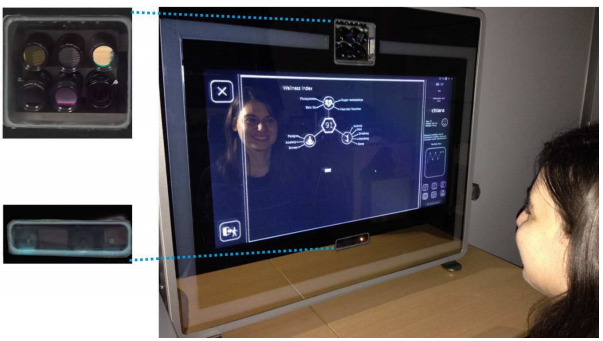
\includegraphics[width=12cm]{images/mirror.png}
    \caption{SEMEOTICONS}
    \label{fig:seme}
\end{figure}
如图 \ref{fig:seme} 所示,Yasmina Andreu-Cabedo等 \cite{andreu2015mirror}则开发了SEMEOTICONS系统。
SEMEOTICONS是一款放在家庭室内环境的镜子,通过摄像头和传感器采集面部信息和体温,监测与心血管疾病相关的疲劳、压力和焦虑等特征, 让用户能够监测自己的健康情况,并根据量身定制的健康指南来改善用户的生活方式。该系统由室内的硬件设备和远程服务器一起完成健康监测的功能,室内设备负责采集数据,远程服务器负责处理数据分析结果。
在生活中照镜子本来就是每个人的日常行为,该研究将读脸技术和健康管理结合起来,并且将应用场景拓展到了日常环境。
他们后续还进行了一次用户体验调研,调研结果表明\cite{coppini2017user} 他们的原型系统的设计被大多数用户所接受: 虽然测试过程非常耗时,大多数参与研究中的志愿者仍然很愿意完成并按计划进行实验,部分志愿者考虑了系统给出的健康指南,甚至因此改变了自己的生活方式。

总的来说,该系统通过将诊断和日常的照镜子的行为结合起来,可以很方便与用户的日常生活融合起来,同时在服务器端也可以方便的实现算法模型的适配和更新。
但是该系统固定在房间的某个位置使用的方式不够便携,同时该系统需要一系列的传感器设备,不仅增加了硬件的成本,部署起来也相对麻烦,而且只能在室内使用。

\section{日常健康管理技术}

由上一节我们知道面诊技术的应用和研究却很少关注日常健康场景,但在人机交互领域,国内外有大量的关于如何设计日常场景下健康相关的交互研究。

从研究目的来看,日常健康技术的研究重心偏向于关注患者的日常生活体验,加强患者与医护人员的协作,提高用户的疾病认知等方面\cite{nunes2015self-care}。
从研究的出发点来看,主要可以分为慢性疾病管理和鼓励用户健康生活方式的研究两种\cite{nunes2015self-care},本小节将从这两个方面展开分别介绍。

\subsection{慢性疾病管理}
随着医学、科技和社会的进步,当前的人们享受着比以往时代更加长寿的生活\cite{OlshanskyDEMOGRAPHY}。寿命的增加也间接地造成了慢性病患病率的提高\cite{kaye2006overview}。慢性病作为一种长期的疾病,大多数在目前的医疗条件下是无法治愈的,但是可以通过适当的管理控制病情,因此慢性病管理变得格外重要\cite{Ben2002A}。

在慢性疾病管理方面,当前研究主要是关于各种类型的慢性疾病的长期管理和追踪技术,用于支持慢性病患者及其护理人员了解病人的身体状态并加强对病情的控制,从而提高用户在患病状态下的生活品质。
如 Lena Mamykina\cite{mamykina2008mahi:}团队在安卓平台上研发了一款称为 MAHI 的应用,通过蓝牙和传统的血糖仪进行通信,
提供了血糖记录的功能,同时为用户开发了对应的Web平台,并且实现了用户之间在平台上互相交流等功能,经过实验发现该系统提供的功能能够大大鼓励用户完成血糖管理的任务(如严格控制饮食)。
Kiyoshi Yasuda等\cite{yasuda2009remote}则研究了如何设计与痴呆病人的远程通讯系统,帮助痴呆病人与家人进行沟通,提高痴呆病人在家保持情绪稳定的时间,改善痴呆病人的日常在家的生活质量。
Amid Ayobi等\cite{ayobi2017quantifying} 通过对多发性硬化病人的日常监测应用的研究,发现日常健康技术可以帮助提高病人的日常控制意识,而不只是监测疾病相关的指标。

在精神健康方面,Jakob E. Bardram等\cite{bardram2013designing}探索了如何设计监测双相情感障碍症的日常应用, 研究发现因为移动平台的便携性,患者可以随时携带智能手机,通过系统提醒和实时数据可视化可以提高患者的疾病意识。
同时该系统提供的评估功能相较于纸质表格评估的模式,使用体验大大得到了提高,更加利于用户长期坚持疾病评估。

总的来说,健康管理和患者的日常生活密切相关,慢性病患者需要调整自己的饮食和锻炼等来实现有效的健康管理\cite{nunes2018understanding}, 因此研究慢性病管理技术对提高慢性病患者的生活水平非常重要。
慢性病管理技术能够帮助用户了解病情的变化,及时对自己的病情变化做出应对行为,更好地评估自己的日常健康行为和更快地适应当前的生活状态\cite{ayobi2017quantifying}。


\subsection{健康行为引导}
在鼓励用户健康生活方面,主要是对各类监测系统的研究。这类系统的功能主要是对用户的各种健康比较相关的指标,能够让用户得到关于自己健康情况的一个反馈,
让处于健康或者亚健康的情况下的用户更加健康地生活。这类监测相关的技术,从对用户监测的指标来看,可以大致分为两类:
\begin{enumerate}

    \item 日常行为的监控:通过监控用户的日常饮食、运动情况等日常行为,培养用户更好的饮食习惯、锻炼习惯等\cite{purpura2011fit4life,Inagawa2013A,bravata2007using,cordeiro2015barriers,lin2006fish, miller2014stepstream}。 例如Yuma Inagawa等人\cite{Inagawa2013A} 开发了一个营养管理和检索系统,根据用户的喜好给出推荐的菜单,用户也可以给出对应的反馈,以此来培养用户健康的健康饮食的观念,进而达到引导用户的行为的效果。


    \item 健康指标的监控:健康指标主要包括生命体征如呼吸、血压、心率,也包括睡眠、体重等\cite{kay2012lullaby,gronvall2013beyond,logan2007mobile,walters2010a}。
    
\end{enumerate}

例如Stephen Purpura等人\cite{purpura2011fit4life} 利用内有传感器的眼镜、耳机,臂环等可穿戴设备,通过记录用户的饮食、心率、咀嚼动作、体重、血压等健康指标,设计了一个鼓励用户减肥的系统 fit4life; 
Lullaby\cite{kay2012lullaby}是Matthew Kay等人利用光线、声音、温度、运动等传感器研发出来,用于研究干扰用户睡眠因素的系统。
Lullaby系统通过记录和可视化用户的睡眠状态,能够帮助用户识别睡眠中断和环境因素之间的联系。 

% 总结上述的研究我们发现,当前关于日常健康交互技术的研究有很多,涉及各种慢性疾病管理以及各种健康评估和监测的方法,但是目前还缺乏关于日常环境下如何设计基于面部信息进行健康评估的研究。

不过目前这些健康追踪和监测技术,主要的实现方式还是通过量化采集用户的健康指标相关的数据。那么如何利用其他的健康相关数据,如面部信息,来支持用户的日常健康,在人机交互领域还没有得到深入研究。



\section{本章小结}
本章主要介绍了当前主要的面诊系统设计已经各自的特点和不足,尤其在日常健康场景的系统设计研究目前还十分欠缺。
而人机交互领域在日常健康方面的研究值得我们借鉴。本章后半段介绍了人机交互领域从传统的慢性疾病管理到支持用户更健康生活方式的研究,同时指出当前的日常健康的研究,还未探索面部信息作为健康指标的技术。

